\section{Coarse-grained simulations}

During the discussion of the nanopiston's operation cycle it was hypothesised
that entropic interactions play an important role in its functioning. Studying these
phenomena is experimentally rather difficult, since all results are deduced from the
measured current traces and known interactions between the different elements of the
system. To obtain a more in-depth understanding of these interactions, computer
simulations are needed to provide the necessary insights.

In view of these challenges, a coarse-grained model of the DNA nanopiston was devised by
Bayoumi et al. The model is used to perform molecular dynamics simulations of  the
conformational fluctuations of the rotaxane at zero bias. Performing the simulations was
done by using the Large-scale Atomic/Molecular Massively Parallel Simulator (LAMMPS) and
its implementation of a Langevin intergrator.[.]

The coarse-grained model is composed of four types of interacting pseudo-atoms, all
taking into account excluded volume interactions via repulsive Lennard-Jones
potentials. First of all, the ClyA nanopore is represented by three vertically stacked
open cylinders, with diameters 6 nm, 5.5 nm and 2.9 nm from the cis- to the trans-side.
To take into account the electrostatic DNA-nanopore interactions, the cylinder radii
are appropriately adjusted from the pore's geometry reported in.[.]
These electrostatic interactions predominantly arise from an excess negative charge in
the constriction of ClyA, resulting in a reduced effective size of the trans-cylinder.
Note that the pore is excluded from the Langevin integration, resulting in a static pore
model.

A semiflexible bead-and-spring model is used to simulate the rotaxane. Each spherical
bead represents one ssDNA nucleotide or five dsDNA base pairs, respectively having a
diameter of $1\ nm$ and  $2.2\ nm$. The bond connecting each consecutive pair of beads is
represented by a harmonic spring. Determining the bond stiffness is done by means of the
equipartition theorem, from which we find
  \begin{equation}
    k_{bond} = \frac{3 k_b T }{ \langle a \rangle},
  \end{equation}
here $\langle a \rangle$ is the equilibrium bond length taken to be $0.68\ nm$ or $1.7\
nm$ for ssDNA and dsDNA respectively. In this model the bending rigidity of the DNA
polymer is taken into account. This effect is modelled as previously seen in the discrete
worm like chain, where the angle between consecutive bond vectors is assigned a harmonic
potential. Using equation .., the bending rigidity is determined by
  \begin{equation}
    \kappa_{bend} = \frac{l_{p} \kappa_b T}{\langle a \rangle},
  \end{equation}
  where $l_p$ is the persistence length of the ssDNA ($2.2\ nm$) or dsDNA ($45\ nm$)
strands. The difference in persistence length results in the relatively large flexibility
of ssDNA.

The last components of the coarse-grained model are the neutravidin protein stoppers,
which capture the rotaxane inside of the nanopore. During experiments it was observed
that the neutravidin proteins can enter the lumen of ClyA. Using this information, the
size of the spherical stoppers was fitted to reproduce this behaviour in simulations.
The fitted value is a diameter of $7\ nm$. The lipid bilayer in which the pore is
embedded also interacts with these proteins, which is implemented by a reflective
boundary at the lower entrance of the nanopore.

Having established a coarse-grained model of the DNA nanopiston, a computational analysis
of the conformational fluctuations can be performed. A first conclusion drawn from these
simulations is the importance of the toehold of rotaxane-ds. It was observed
that the toehold was kept outside of the constriction of ClyA, resulting from the high
entropic cost of confining the flexible strand of ssDNA. This affinity of the toehold to
be outside of the nanopore exposes it for initiating the strand displacement, even if an
opposing bias is applied.

The hybridisation of rotaxane-ss is also supported by entropic interactions. The
interface between the ssDNA and dsDNA parts is kept outside of the nanopore, resulting
from the entropic cost of confining the dsDNA in the constriction of ClyA. Keeping the
interface outside of the pore prevents the sequestering of the toehold during
hybridisation.

These simulations clearly highlight the importance of entropic interactions between the
DNA rotaxane and the nanopore during the piston's operation cycle. However, the model
used by Bayoumi et al.[.] imposes limitations on the possible research that can be
performed. More advanced methods are needed, which are discussed in the following
chapters of the thesis.\\\\


\begin{figure}[ht]
  \begin{centering}
  \adjustbox{minipage=1.3em,valign=t}{\subcaption{}\label{sfig:testa}}%
  \begin{subfigure}[t]{\dimexpr.4\linewidth-1.3em\relax}
  \centering
  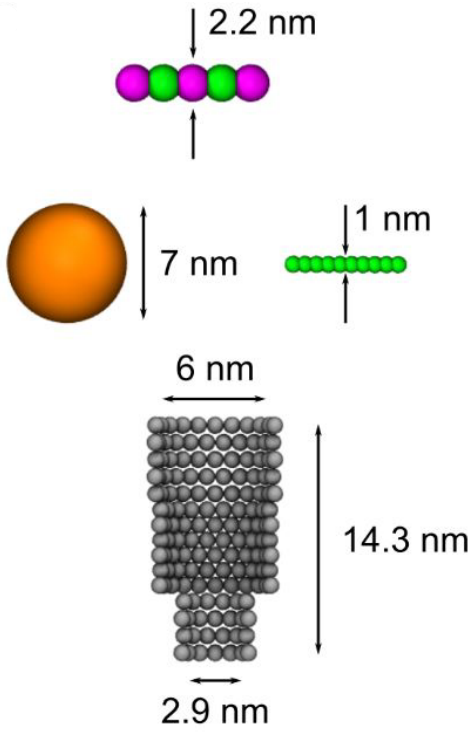
\includegraphics[width=0.9\linewidth,valign=t]{Figures/Stefanos1.png}
  \end{subfigure}%
  \adjustbox{minipage=1.3em,valign=t}{\subcaption{}\label{sfig:testb}}%
  \begin{subfigure}[t]{\dimexpr.5\linewidth-1.3em\relax}
  \centering
  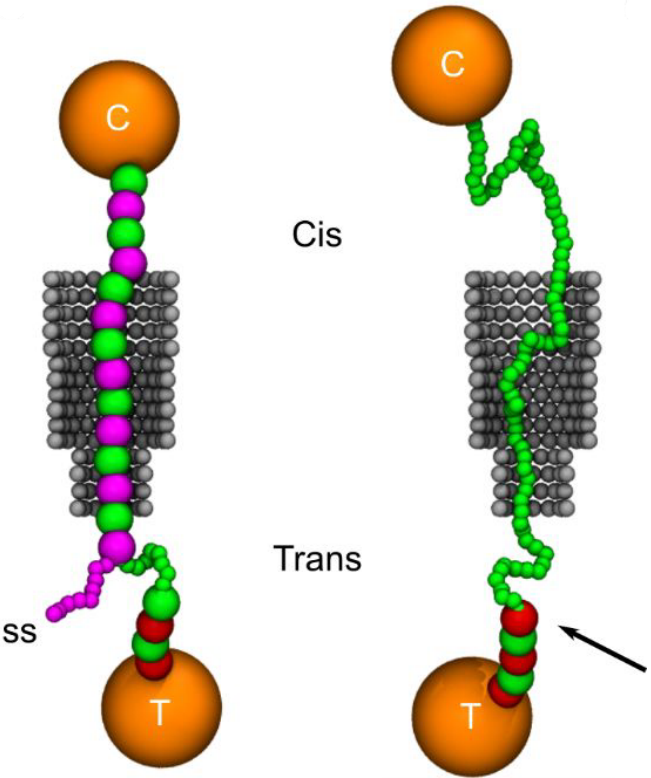
\includegraphics[width=0.9\linewidth,valign=t]{Figures/Stefanos2.png}
  \end{subfigure}
  \caption{This is a figure}
  \label{fig:test}
  \end{centering}
\end{figure}

